\section{Diagrammi di Sequenza}
\label{sec:Diagrammi di Sequenza}

In questa sezione saranno riportati i diagrammi di sequenza riguardo alle operazioni dell'applicazione ritenute significative che descrivono le interazioni tra attori ed oggetti o entità di sistema.

\subsection{Richiesta lista edifici abilitati}
\label{sub:Richiesta lista edifici abilitati}

\begin{figure}[!h]
	\centering
   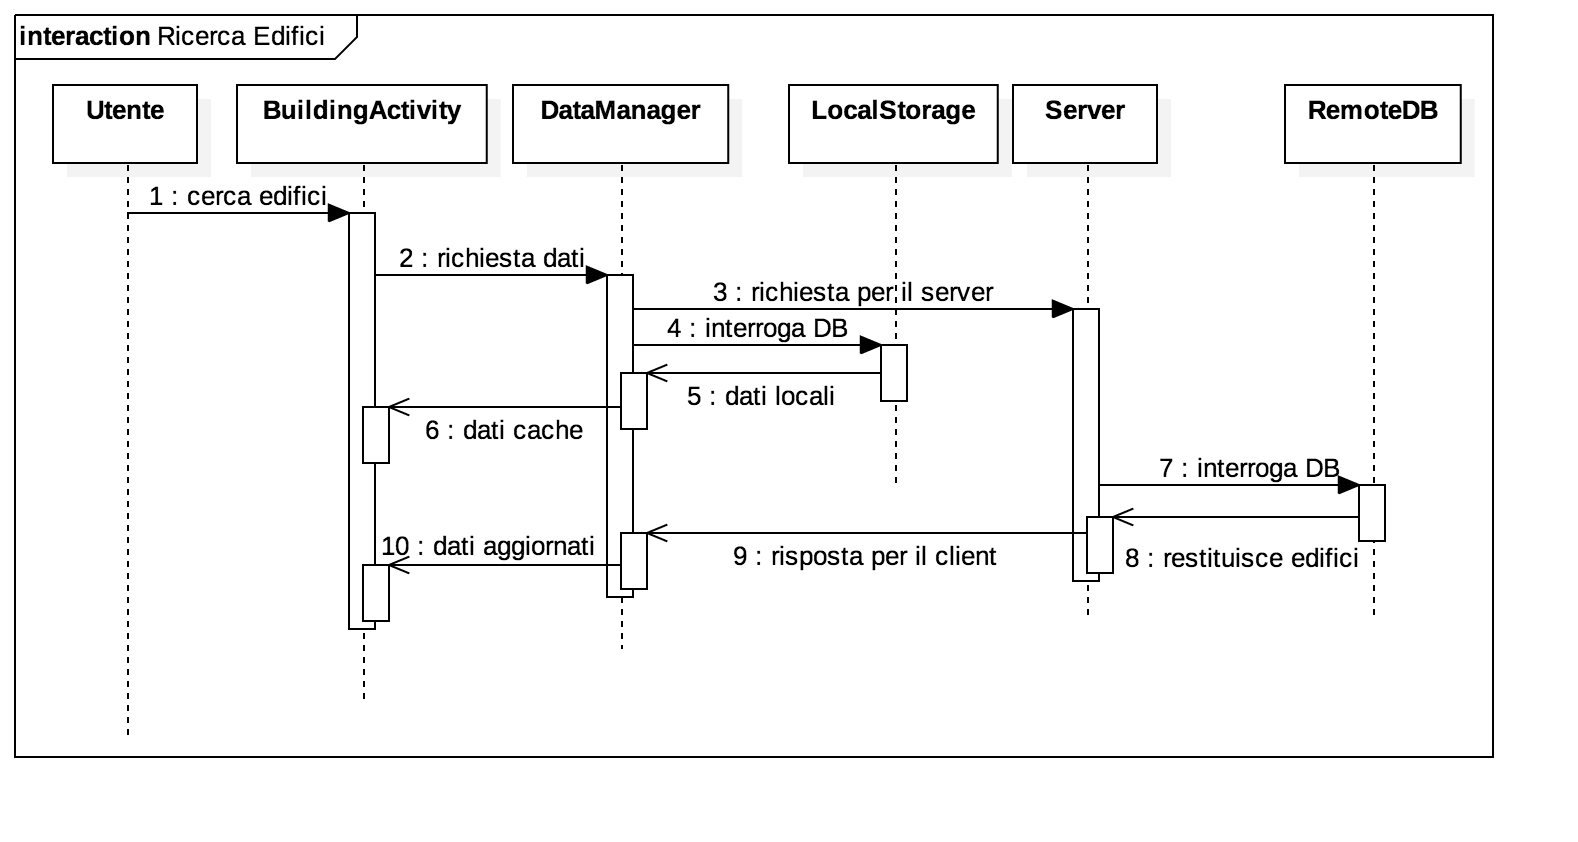
\includegraphics[scale=0.28]{img/diagrammiSequenza/ricercaEdifici.png}
   \caption{Diagramma di Sequenza della richiesta di edifici abilitati ai percorsi}
\end{figure}

Il diagramma in figura illustra come viene gestita la visualizzazione nel client della lista di edifici abilitati nelle vicinanze.
La sequenza ha inizio ogni volta che l'utente accede alla schermata di ricerca degli edifici abilitati dal proprio terminale.

L'activity che si occupa di gestire la lista degli edifici (\texttt{BuildingsActivity}) richiede i dati attraverso la classe \texttt{DataManager}, situata nel package \texttt{CLIPS::data::datamanager}.
A questo punto il \texttt{DataManager} interrogherà sia il database locale alla ricerca di dati in cache (per fornire nel più breve tempo possibile i dati all'utente), sia il server (per ottenere i dati più aggiornati).
Solitamente il database locale risponderà in tempi brevissimi, ritornando quindi l'informazione richiesta al \texttt{DataManager} che provvederà a inviarla alla activity che l'ha richiesta.
Intanto la richiesta inviata al server viene instradata dal \texttt{Server} alla corretta classe che si occuperà di interrogare il DB remoto per ottenere i dati più aggiornati.
Tali dati vengono poi inviati dal server fino al \texttt{DataManager} e poi di nuovo all'activity, che avrà ora i dati più aggiornati da mostrare all'utente.

\subsection{Scoperta nuovi \gl{Beacon}}
\label{sub:Scoperta nuovi Beacon}

\begin{figure}[!h]
	\centering
   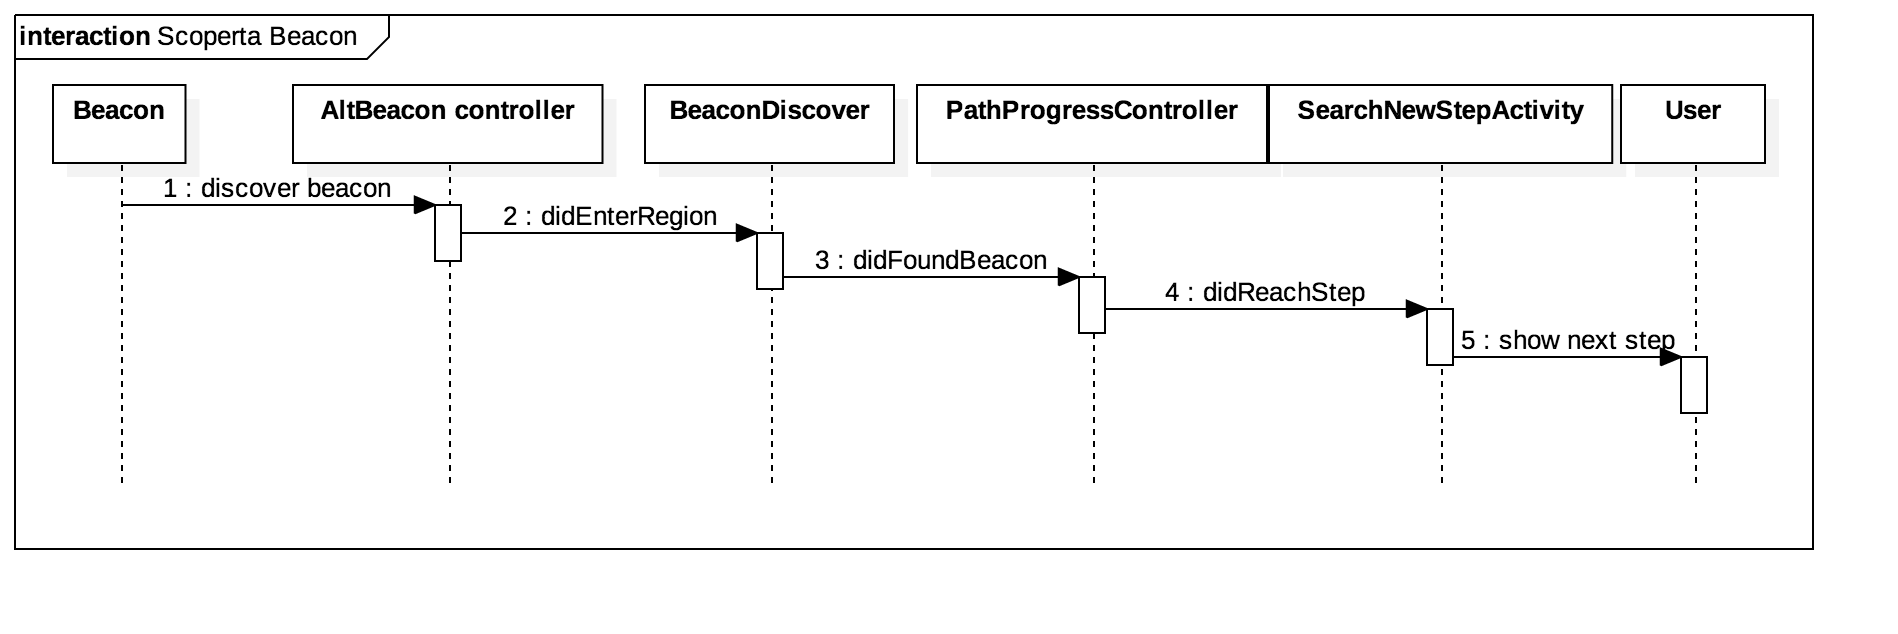
\includegraphics[scale=0.22]{img/diagrammiSequenza/scopertaBeacon.png}
   \caption{Diagramma di Sequenza della scoperta di nuovi beacon}
\end{figure}

Il diagramma in figura illustra come viene gestita dall'app la situazione in cui, durante lo svolgimento di un percorso, l'utente si avvicini al \gl{beacon} che segnala il raggiungimento della prova seguente.

Il \gl{beacon} trasmette costantemente i propri dati nelle vicinanze; quando il dispositivo ne rivela la presenza lo segnala all'applicazione attraverso la libreria \gl{AltBeacon} che effettua una chiamata al metodo \texttt{didEnterRegion} di un oggetto di tipo \texttt{BeaconDiscover}.
A sua volta il \texttt{BeaconDiscover} chiamerà il metodo \texttt{didFoundBeacon} nel proprio delegate (ovvero un istanza di \texttt{PathProgressController}) che si occuperà di capire se il \gl{beacon} è effettivamente uno del percorso ed eventualmente notificarlo all'activity \texttt{SearchNewStepActivity} che ha il compito di informare l'utente.
